%%%% fatec-article.tex, 2024/03/10

\documentclass[
  a4paper,%% Tamanho de papel: a4paper, letterpaper (^), etc.
  12pt,%% Tamanho de fonte: 10pt (^), 11pt, 12pt, etc.
  english,%% Idioma secundário (penúltimo) (>)
  brazilian,%% Idioma primário (último) (>)
]{article}

%% Pacotes utilizados
\usepackage[]{fatec-article}

%% Início do documento
\begin{document}
\vspace{8cm}
\begin{center}
    \large \textbf{\title{ARTEFATOS DO PROJETO DE SOFTWARE}}
\end{center}

\maketitle

\break

\tableofcontents

\break


%exemplo da forma de organização das seções e subseções, você deverá adaptar o template para a realidade do seu projeto.

\section*{Diagramas UML}
    Nesta seção serão apresentados os diagramas da UML utilizados para a modelagem do sistema desenvolvido. Dentre os diagramas utilizados, pode-se citar: Diagrama de Caso de Uso, Diagrama de Classe e Diagrama de Objetos.
    
    \subsection*{Diagrama de Caso de Uso}
    \addcontentsline{toc}{section}{Diagrama de Caso de Uso}

    Este diagrama de caso de uso aborda o produtor agrícola como principal ator do sistema. 
    A funcionalidade principal do sistema consiste na classificação de fotos de tangerina ponkan para identificação de possíveis sintomas da pinta preta dos citros, sejam as fotos capturadas pelo próprio aplicativo ou carregadas da galeria do dispositivo.
    

    
            \begin{figure}[h]
\centering
\caption{Diagrama de caso de uso}%
\label{fig:diagrama-caso-uso}
 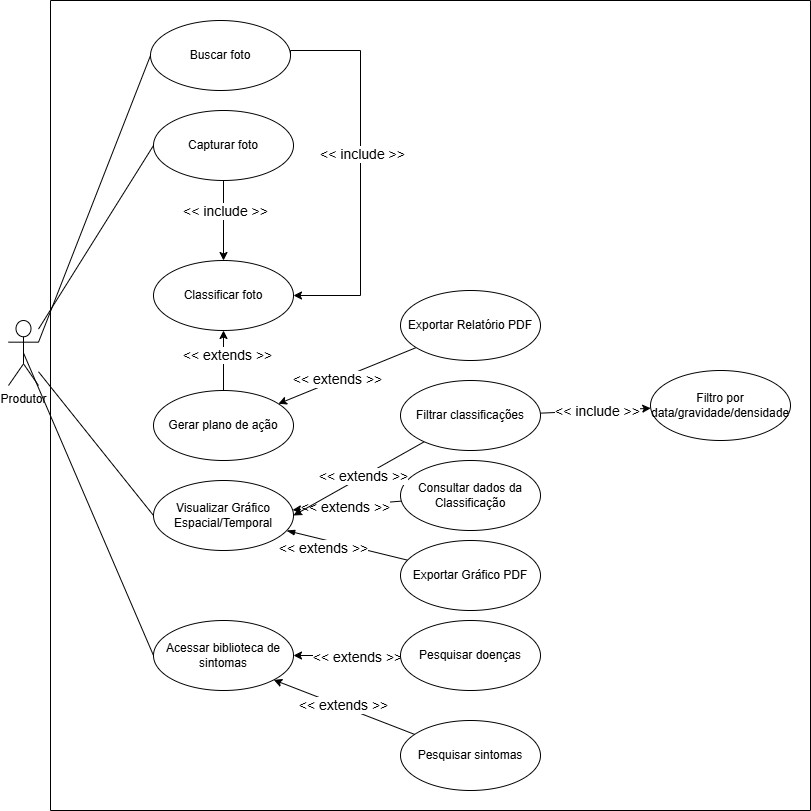
\includegraphics[width=0.8\textwidth]{Logos/caso_de_uso_blackspot.png}
\SourceOrNote{Do próprio autor (2025)}
\end{figure}

    A classificação da foto pode gerar ou atualizar um plano de ação com recomendações de manejo para o produtor, o qual também pode ser exportado no formado de arquivo PDF.

    O conjunto de classificações realizadas pelo usuário também é usado para construir dois tipos de gráficos para visualização: espacial (gráfico de pontos que representam as coordenadas das fotos que foram capturadas e analisadas) e temporal (linha do tempo que prioriza a datação das classificações). 
    Esses mesmos gráficos podem ser exportados para o formato de arquivo PDF. O produtor também pode aplicar filtros para visualizar classificações apenas de um determinado período, com um nível específico de gravidade da doença ou apenas focos locais de infecções.
    Os dados de cada classificação podem ser consultados individualmente nesta mesma seção. 

    Além disso, o sistema vai oferecer uma biblioteca estática com fotos e descrições de doenças e sintomas que ocorrem na tangerina ponkan, na qual o usuário pode pesquisar por informações específicas. Essa seção tem a finalidade de servir como uma consulta rápida ao produtor, destacando as diferenças entre a pinta preta e problemas fitossanitários que podem se assemelhar.

    \subsection*{Diagrama de Classes}
    \addcontentsline{toc}{section}{Diagrama de Classes}

    O diagrama de classes oferece uma visão geral do sistema, mostrando mais detalhes sobre as entidades que participam do seu fluxo de funcionamento.
    
    


    \begin{figure}[h]
\centering
\caption{Diagrama de classes}%
\label{fig:diagrama-classe}
 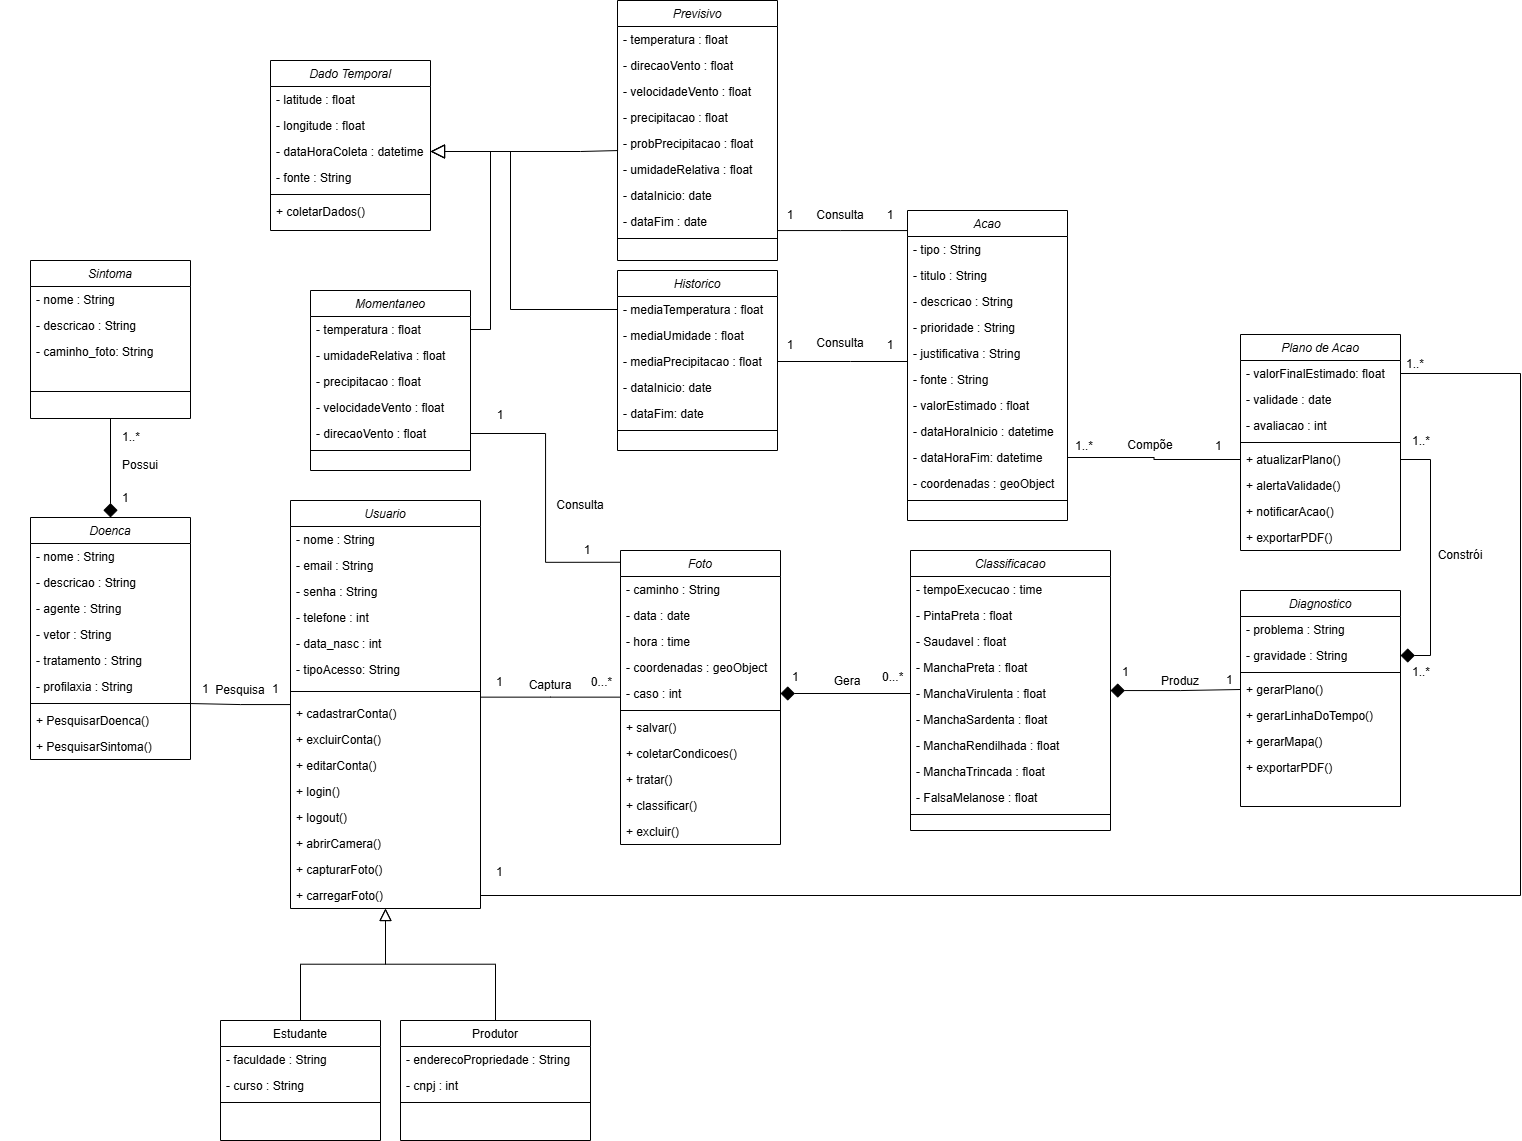
\includegraphics[width=1.0\textwidth]{Logos/classes_blackspot.png}
\SourceOrNote{Do próprio autor (2025)}
\end{figure}

    A classe Usuário possui duas especializações: produtor e estudante, que representam usuários com propósitos diferentes no sistema, embora as funções sejam as mesmas para ambos.
    Suas contas são autenticadas via e-mail e senha.

     Os usuários podem pesquisar doenças e seus sintomas na seção da Biblioteca de Doenças, com cada doença possuindo seus respectivos sintomas.

     Usuários podem capturar (ou carregar) fotos de amostras das frutas. É essencial a utilização de dados como data, hora e coordenadas do local em qua foto foi capturada. 
     O atributo "caso" serve para agrupar fotos de uma mesma amostra, tendo em vista que o usuário poderá capturar até 4 fotos seguidas para classificar - essa foi a alternativa encontrada para agrupar fotos relacionadas sem precisar de uma nova classe ou entidade específica.

     Quando as fotos são tratadas e enviadas para processamento, a rede neural retorna dados que alimentarão a classe chamada Classificação. Ela trata de guardar os valores brutos encontrados pela Inteligência Artificial, como tempo de execução e probabilidade de infecção para cada sintoma da pinta preta.

     Classificações são formalizadas em pré-diagnósticos que podem ser exportados em PDF e servem para alimentar os gráficos e o plano de ação do usuário.

     O plano de ação serve para orientar o produtor sobre o manejo das infecções identificadas, sendo parte fundamental que agrega valor ao sistema. Através de dados climáticos extraídos de APIs e um conjunto de regras que são definidas pela classe Ação, o plano de ação organiza uma lista personalizada de controle e prevenção que o produtor também pode exportar em PDF.
     
     O plano de ação é atualizado toda vez que um novo pré-diagnóstico é gerado, ou pelo próprio usuário, que pode atualizar o plano apenas com base em novos dados climáticos. 

     A classe Dado Temporal trata dados climáticos extraídos de APIs, podendo ser especializada em dados históricos e previsivos (que alimentam o plano de ação) ou em dados momentâneos (que são associados a uma foto no instante da sua captura). A base das recomendações inteligentes do sistema são os dados climáticos.


    \subsection*{Diagrama de Objetos}
    \addcontentsline{toc}{section}{Diagrama de Objetos}

    O diagrama de objetos segue as definições do diagrama de classes e oferece uma visão ainda mais detalhada do funcionamento do sistema, principalmente com relação a implementação.

    É possível notar a diferença entre as coordenadas das fotos com as coordenadas dos dados temporais. Para otimizar a parte lógica do sistema, será utilizado o tipo de dado conhecido como geoObject para armazenar diferentes tipos de localizações - pontos, linhas e polígonos - para fins como a localização de uma foto ou a construção do gráfico de pontos. Já no caso dos dados temporais, como APIs climáticas normalmente entregam respostas com campos latitude e longitude, o sistema também vai usar esses atributos. 

    Note que as fotos se relacionam apenas com dados temporais momentâneos, pois os outros tipos de dados temporais são usados apenas para gerar o plano de ação.

    Também note que, como os objetos da classe Foto possuem diferentes valores no campo "caso", eles dão origem a classificações diferentes e, por consequência, planos de ação distintos.

    Entre os dois planos de ação exemplificados no diagrama, o objeto "plan1" pode ser considerado o plano de ação vigente do usuário, pois a foto que o originou (ft1) é mais recente que a outra (ft2).

    Com relação ao plano de ação, o atributo "avaliação" serve para armazenar a opinião do usuário sobre a qualidade de todo o fluxo principal do sistema: o pré-diagnóstico e as recomendações originadas da foto escolhida. Note que mais de uma ação pode estar associada ao mesmo plano de ação, e que os custos estimados em cada ação são totalizados no plano. 

    Os atributos "fonte" servem para armazenar as referências dos dados que o sistema entrega ao usuário, como a Rede Neural Artificial, APIs climáticas e regras de negócio. Por sinal, as regras de negócio se referem às práticas de manejo e serão estabelecidas com base em estudos científicos sobre o manejo da tangerina ponkan, ou seja, mais tarde fontes externas serão referenciadas, como por exemplo a Embrapa.  


        \begin{figure}[h]
\centering
\caption{Diagrama de objetos}%
\label{fig:diagrama-objetos}
 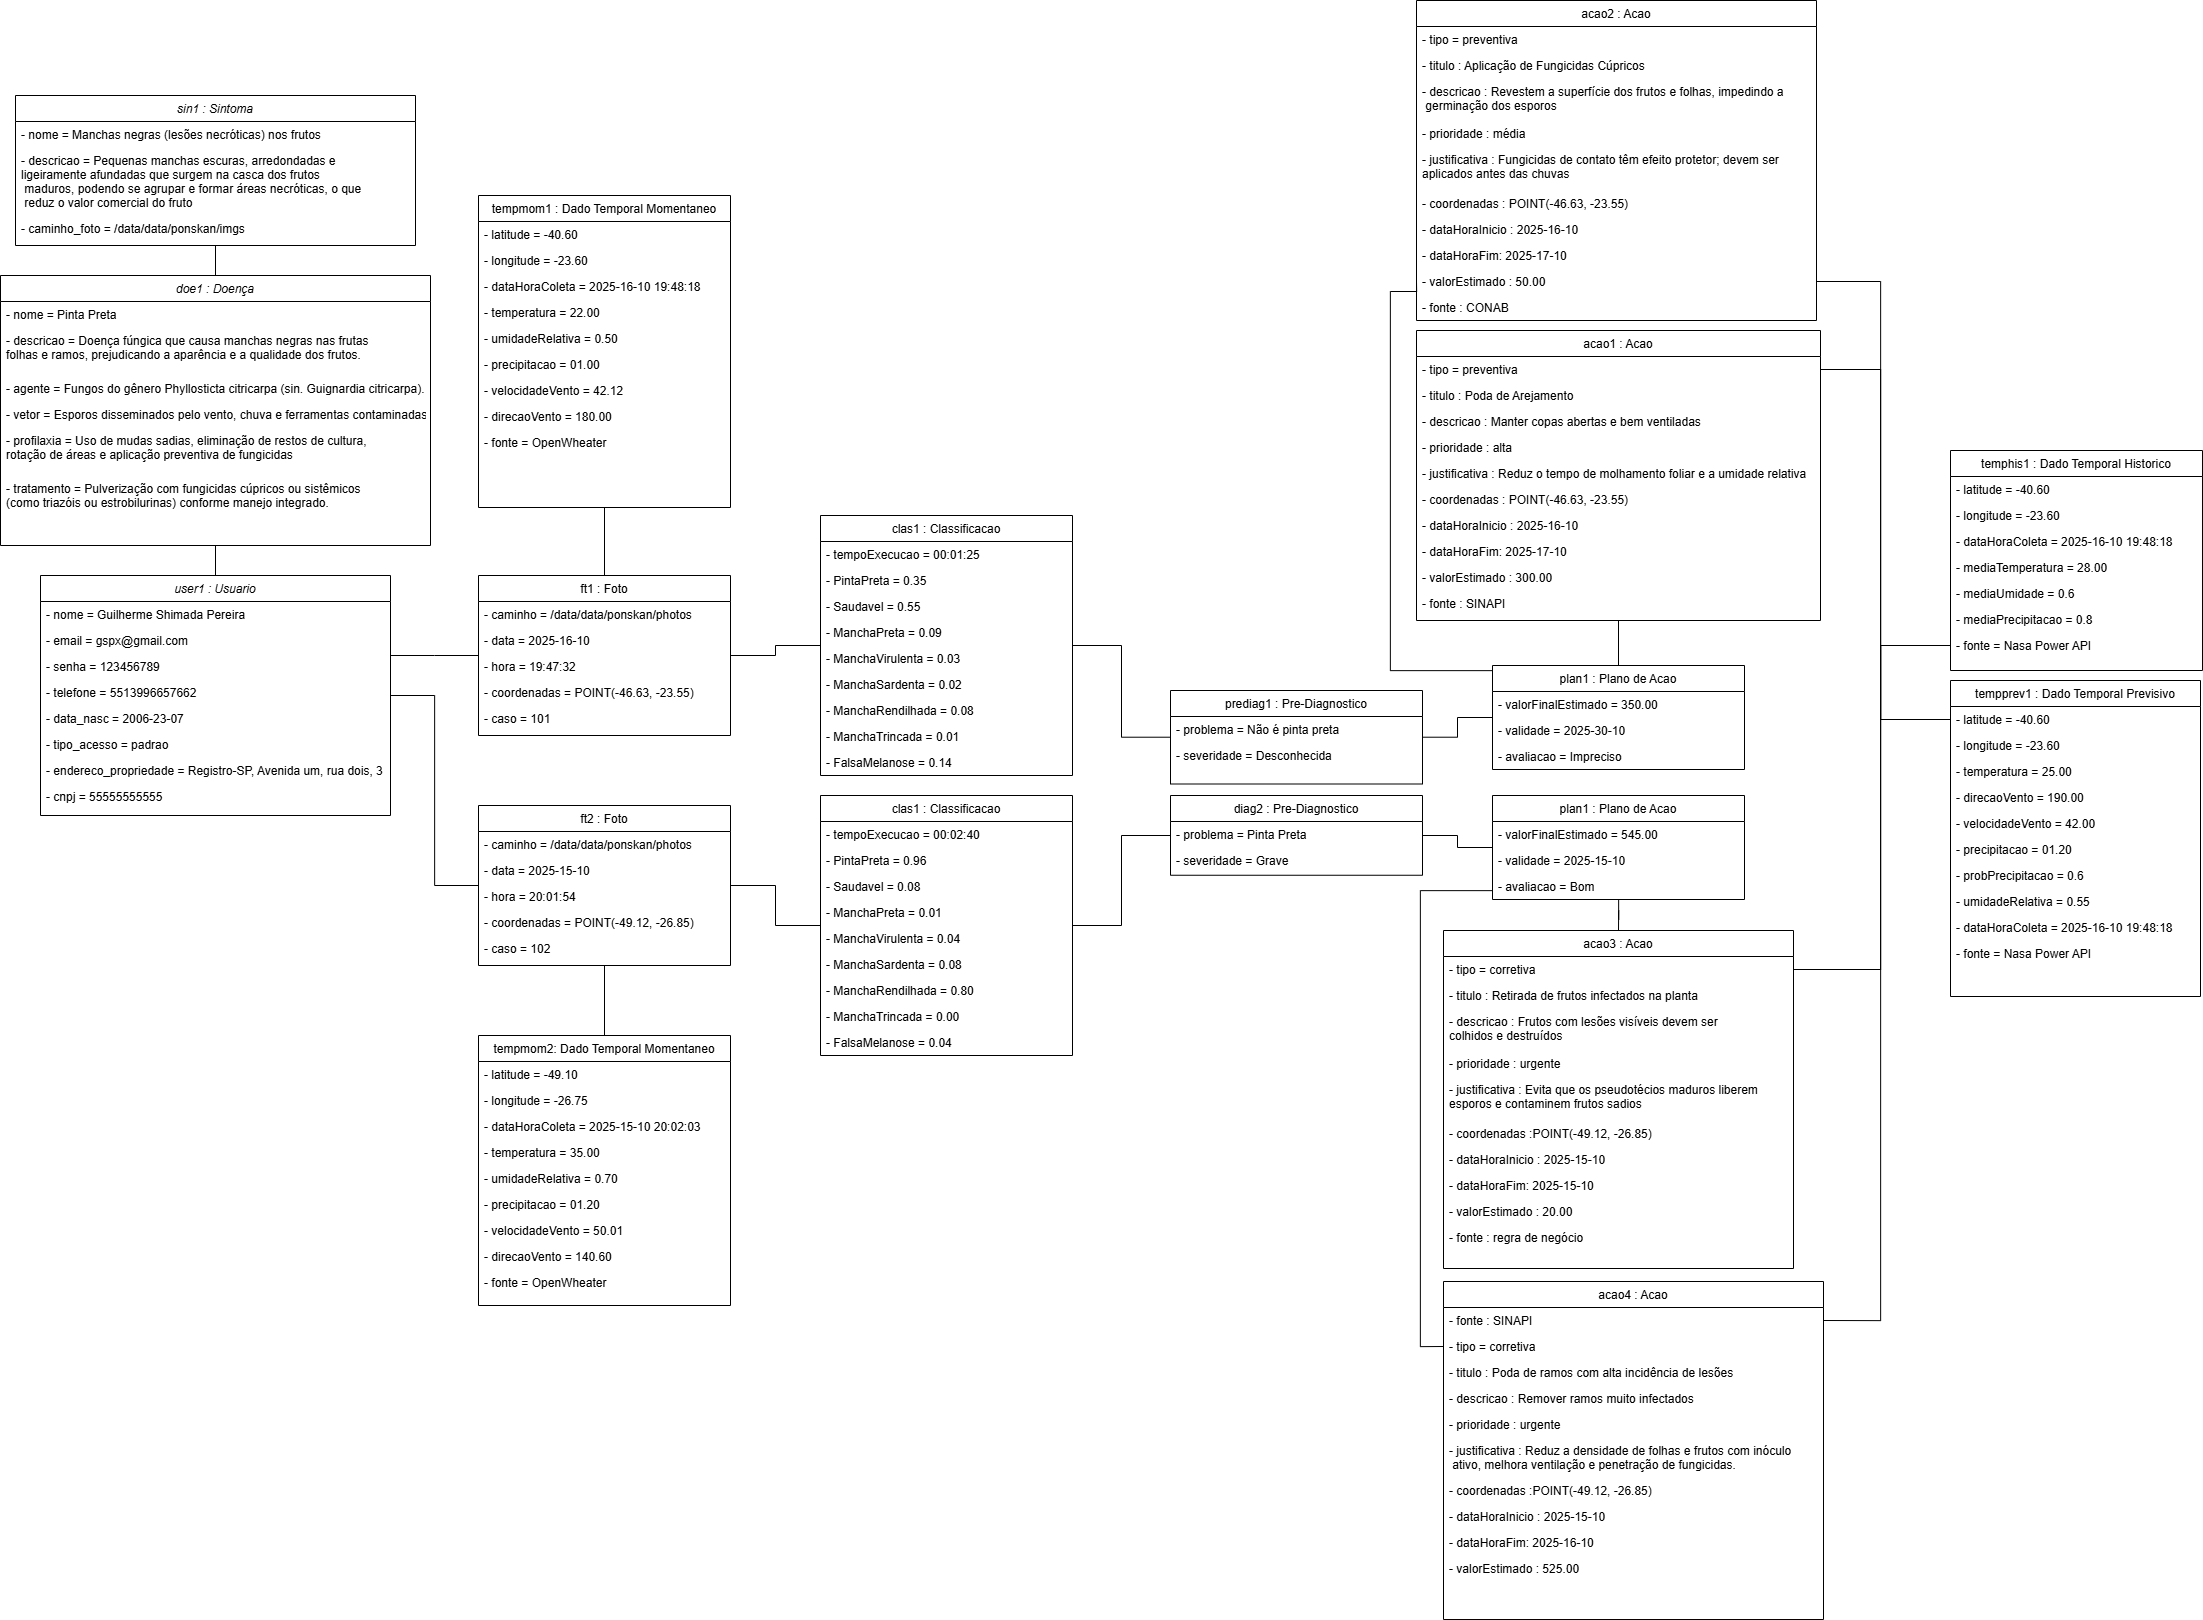
\includegraphics[width=0.8\textwidth]{Logos/objetos_blackspot.png}
\SourceOrNote{Do próprio autor (2025)}
\end{figure}

Por fim, é importante destacar que os objetos "sin1" e "doe1", relativos à seção de Biblioteca de Doenças, possuirão informações estáticas que serão apenas filtradas pelo usuário.

\subsection*{Canvas Business Model}
    \addcontentsline{toc}{section}{Canvas Busines Model}

    O modelo de negócio canvas foi desenvolvido para compreender o projeto da perspectiva administrativa, como uma empresa de potencial competitivo, mapeando as características do negócio.

    Primeiramente, é fundamental compreender que o segmento de clientes do projeto está envolvido na área agrícola e de pesquisa científica, sendo os produtores de ponkan o alvo principal do software, mas também podendo alcançar cooperativas, consultorias e até instituições de pesquisa, que se relacionam com o usuário do tipo estudante.

    O relacionamento dos clientes se daria por treinamentos, canais de suporte e até mesmo uma comunidade digital para produtores de citros. Os meios de comunicação empresa-cliente seriam principalmente digitais. 

    A proposta de valor do aplicativo se baseia na ideia de auxílio ao produtor na identificação precoce da doença da pinta preta, gerando relatórios e recomendações inteligentes que agregam ainda mais valor ao produto. A proposta de valor pode ser traduzida e simplificada em inserir ferramentas de visão computacional no manejo de pequenos e médios produtores, tendo em vista que grandes proprietários optam por tecnologias mais avançadas de controle fitossanitário e prevenção de doenças.

    Para concretizar a proposta de valor, a empresa realiza atividades que envolvem o desenvolvimento da plataforma e do modelo de inteligência artificial. Os recursos se resumem a infraestrutura, equipe, banco de dados e software. 

    As possíveis parcerias estão na mesma área do segmento de clientes.

    Os principais custos que a empresa arcaria seriam relacionados ao desenvolvimento e manutenção do sistema. 
    


        \begin{figure}[h]
\centering
\caption{Canvas Business Model}%
\label{fig:diagrama-objetos}
 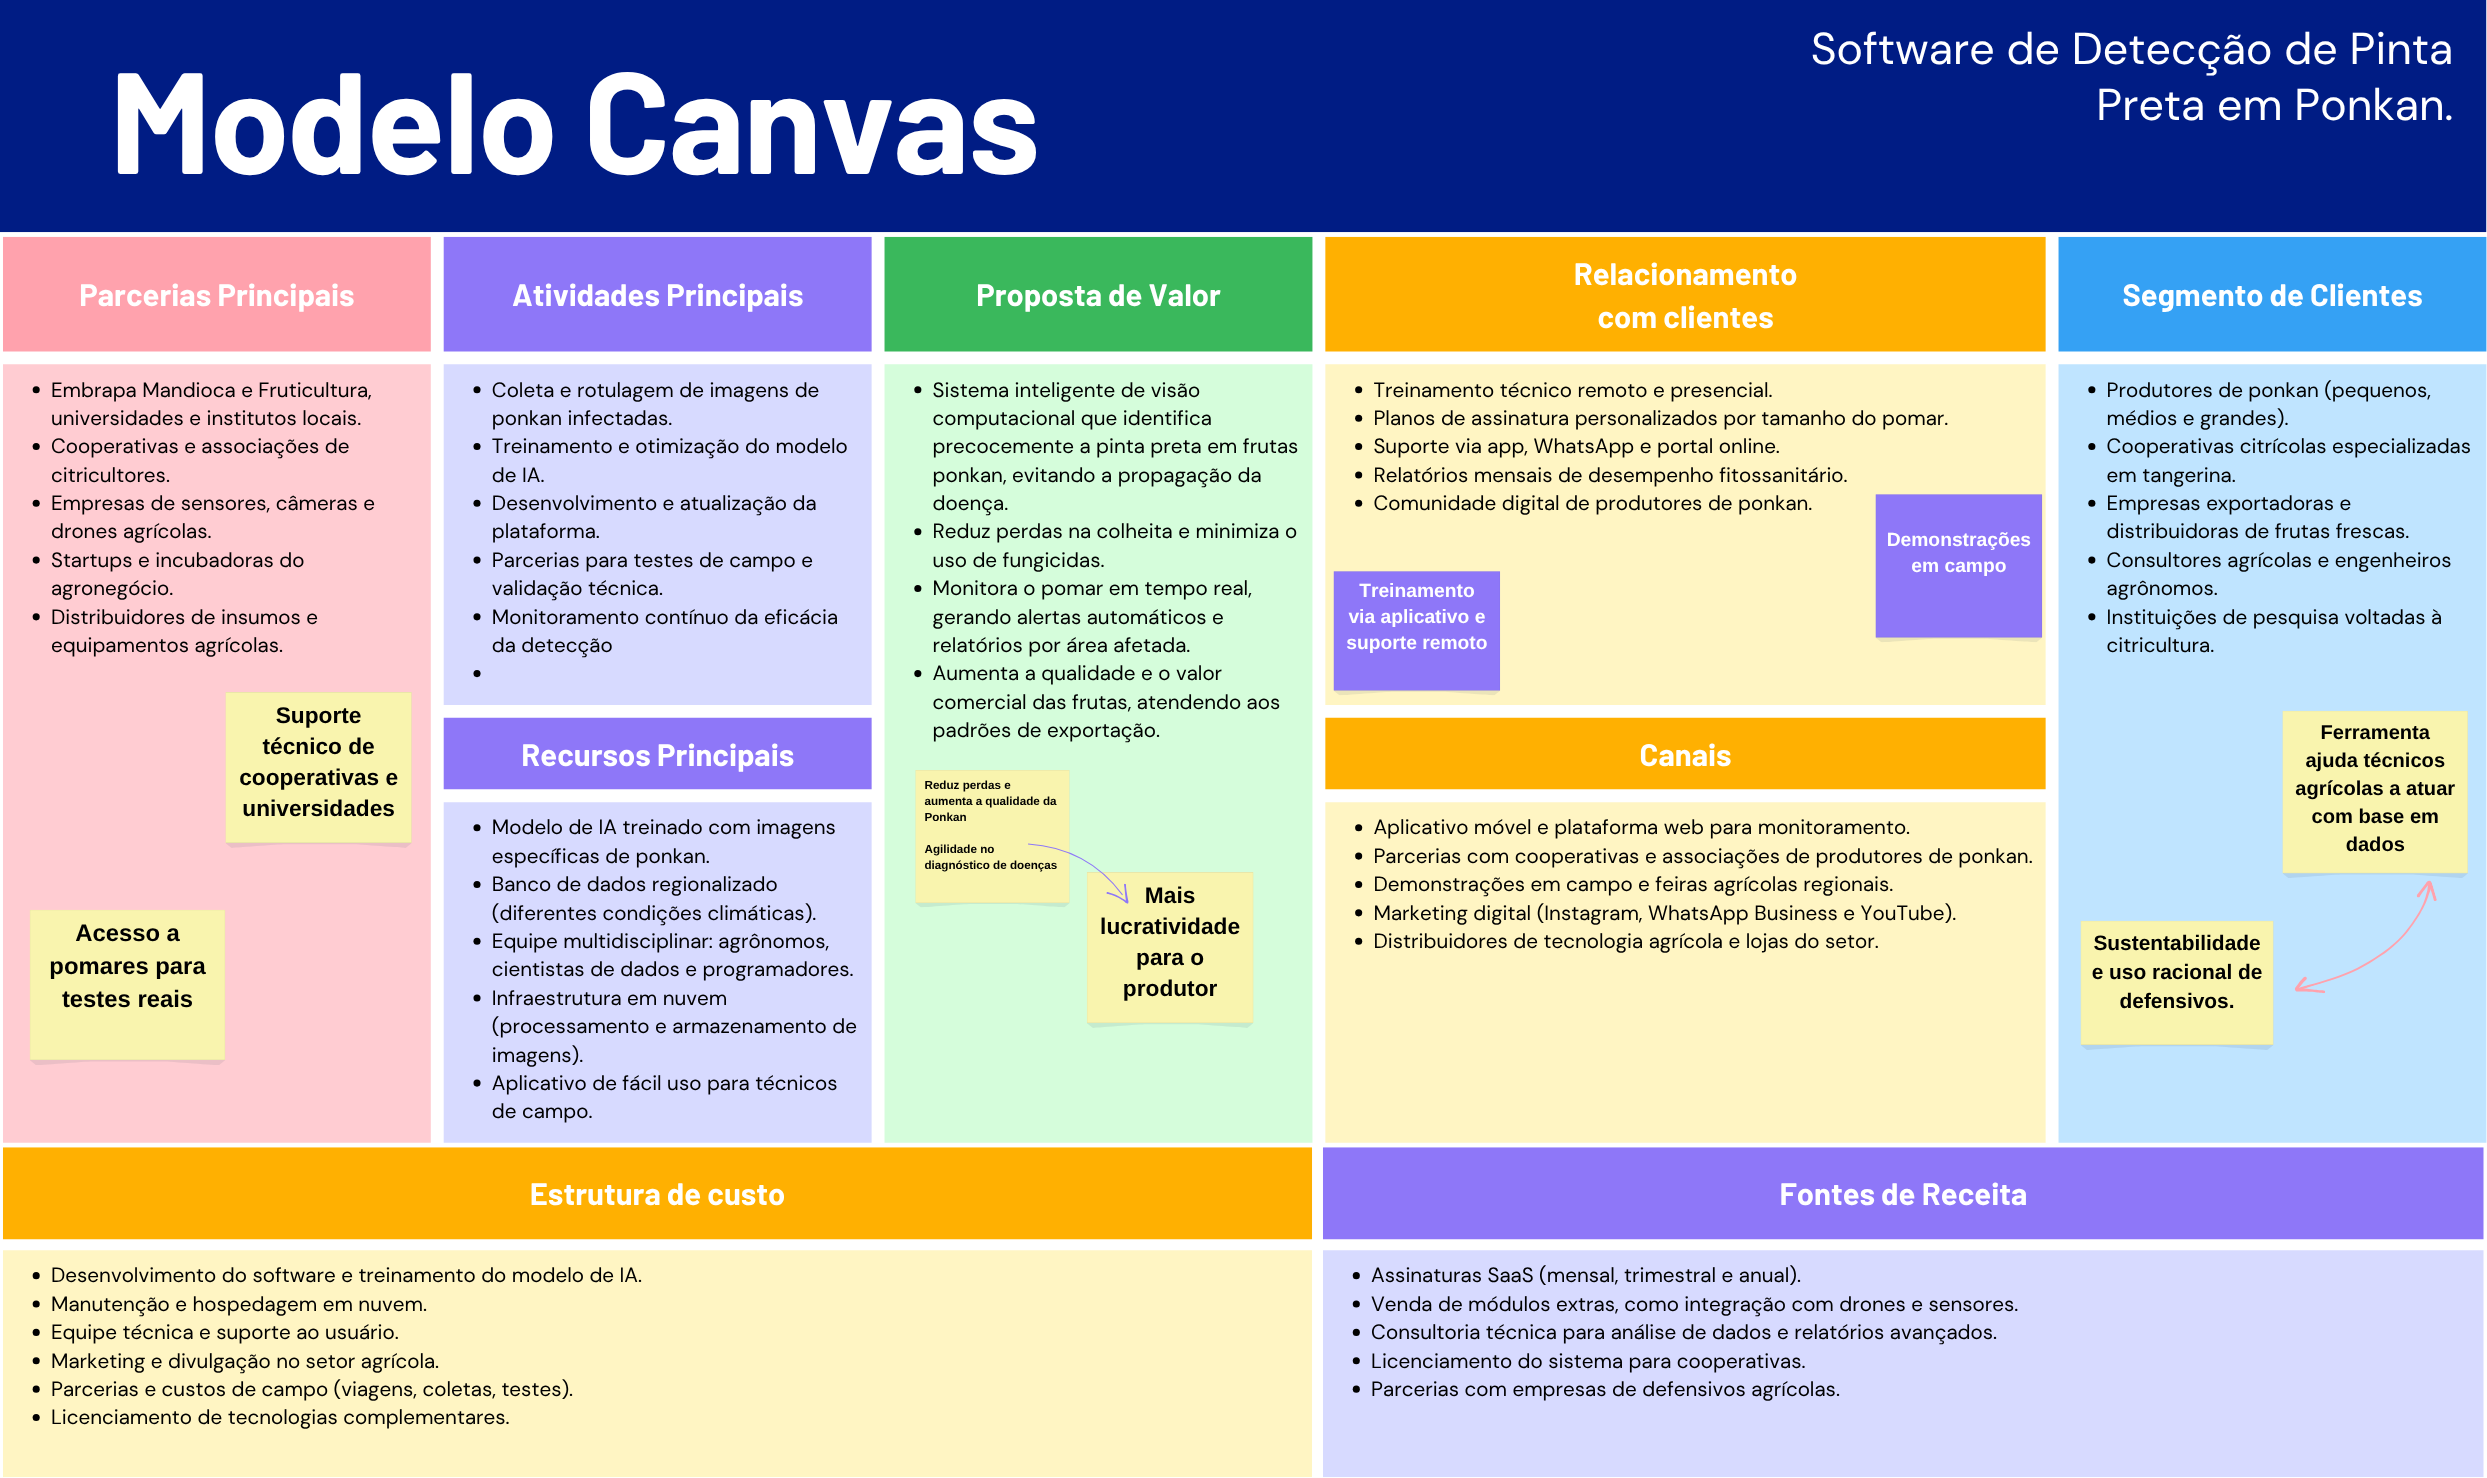
\includegraphics[width=0.9\textwidth]{Logos/canvas.png}
\SourceOrNote{Do próprio autor (2025)}
\end{figure}

Por fim, a forma de receita focaria em assinaturas adaptadas a diferentes realidades dos produtores, venda de módulos adicionais do sistema e outros processos que envolvem parcerias.

\subsection*{Modelo conceitual do banco de dados}
    \addcontentsline{toc}{section}{Modelo conceitual do banco de dados}

    O modelo conceitual do banco de dados apresenta uma visão da perspectiva do armazenamento de dados.

    A entidade usuários agrupa todos os atributos das especializações estudante e produtor, descritas no diagrama de classes. Já no outro caso parecido, dos dados temporais, foi decidido manter tabelas separadas para facilitar a organização e as consultas necessárias.
    
    Novamente, fica visível que a entidade de fotos interage apenas com dados temporais consultados no instante em que a foto é capturada, já as ações do plano de ação consultam os registros climáticos históricos e de previsão, fazendo-se necessária uma entidade associativa de consulta.
    
    Com relação ao plano de ação em si, é importante destacar a relação 1 para 1 com a entidade usuário, e 1 para muitos com a entidade pré-diagnósticos. Isso significa que o usuário possui um único plano de ação  que pode ser atualizado por vários pré-diagnósticos.
    
    A entidade pesquisa biblioteca foi criada para intermediar os filtros que o usuário aplica sobre a seção da Biblioteca de Doenças. 

    Vale destacar que, como o pré-diagnóstico é apenas uma formlização da entidade classificação, ela foi posta como entidade mais fraca desse relacionamento.

        \begin{figure}[h]
\centering
\caption{Modelo conceitual do banco de dados}%
\label{fig:diagrama-objetos}
 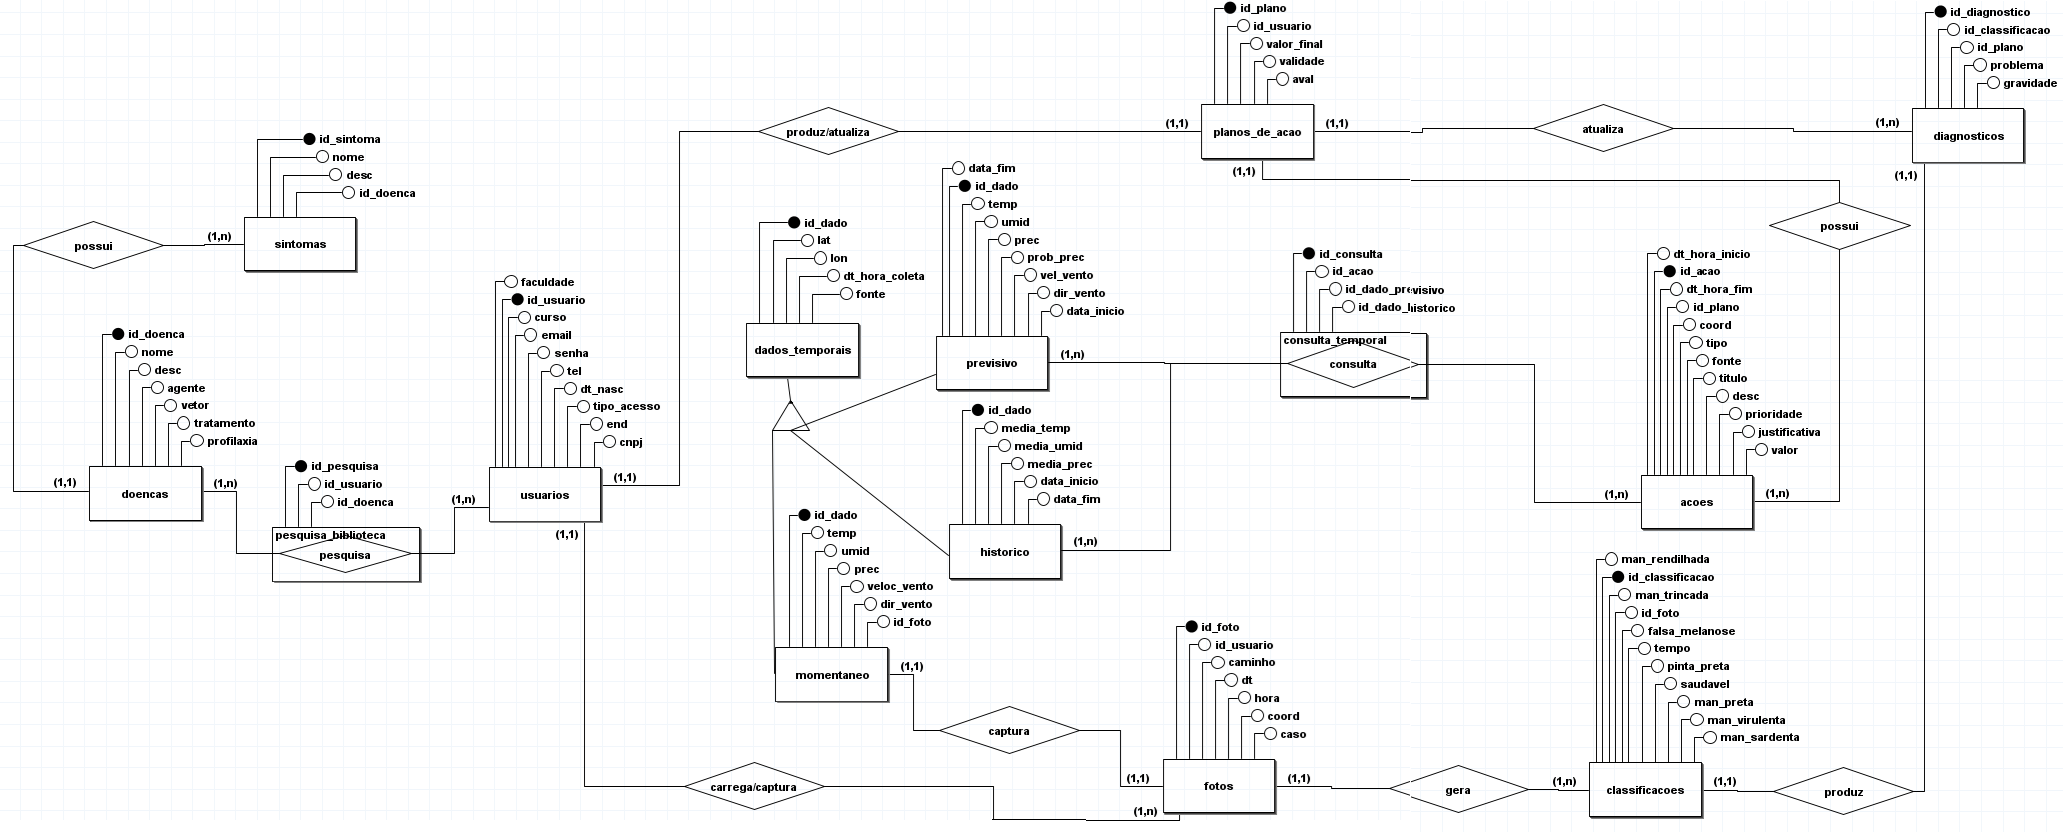
\includegraphics[width=1.1\textwidth]{Logos/conceitual.png}
\SourceOrNote{Do próprio autor (2025)}
\end{figure}


Mais uma vez, é possível identificar de forma clara que as funcionalidades principais do sistema estão concentradas e dependem principalmente dos dados temporais e das fotos capturadas pelo usuário.

\subsection*{Modelo lógico do banco de dados}
    \addcontentsline{toc}{section}{Modelo lógico do banco de dados}

    O modelo lógico do banco de dados permite visualizar os tipos de dados que serão armazenados, os quais correspondem ao indicado no diagrama de classes.

            \begin{figure}[h]
\centering
\caption{Modelo lógico do banco de dados}%
\label{fig:diagrama-objetos}
 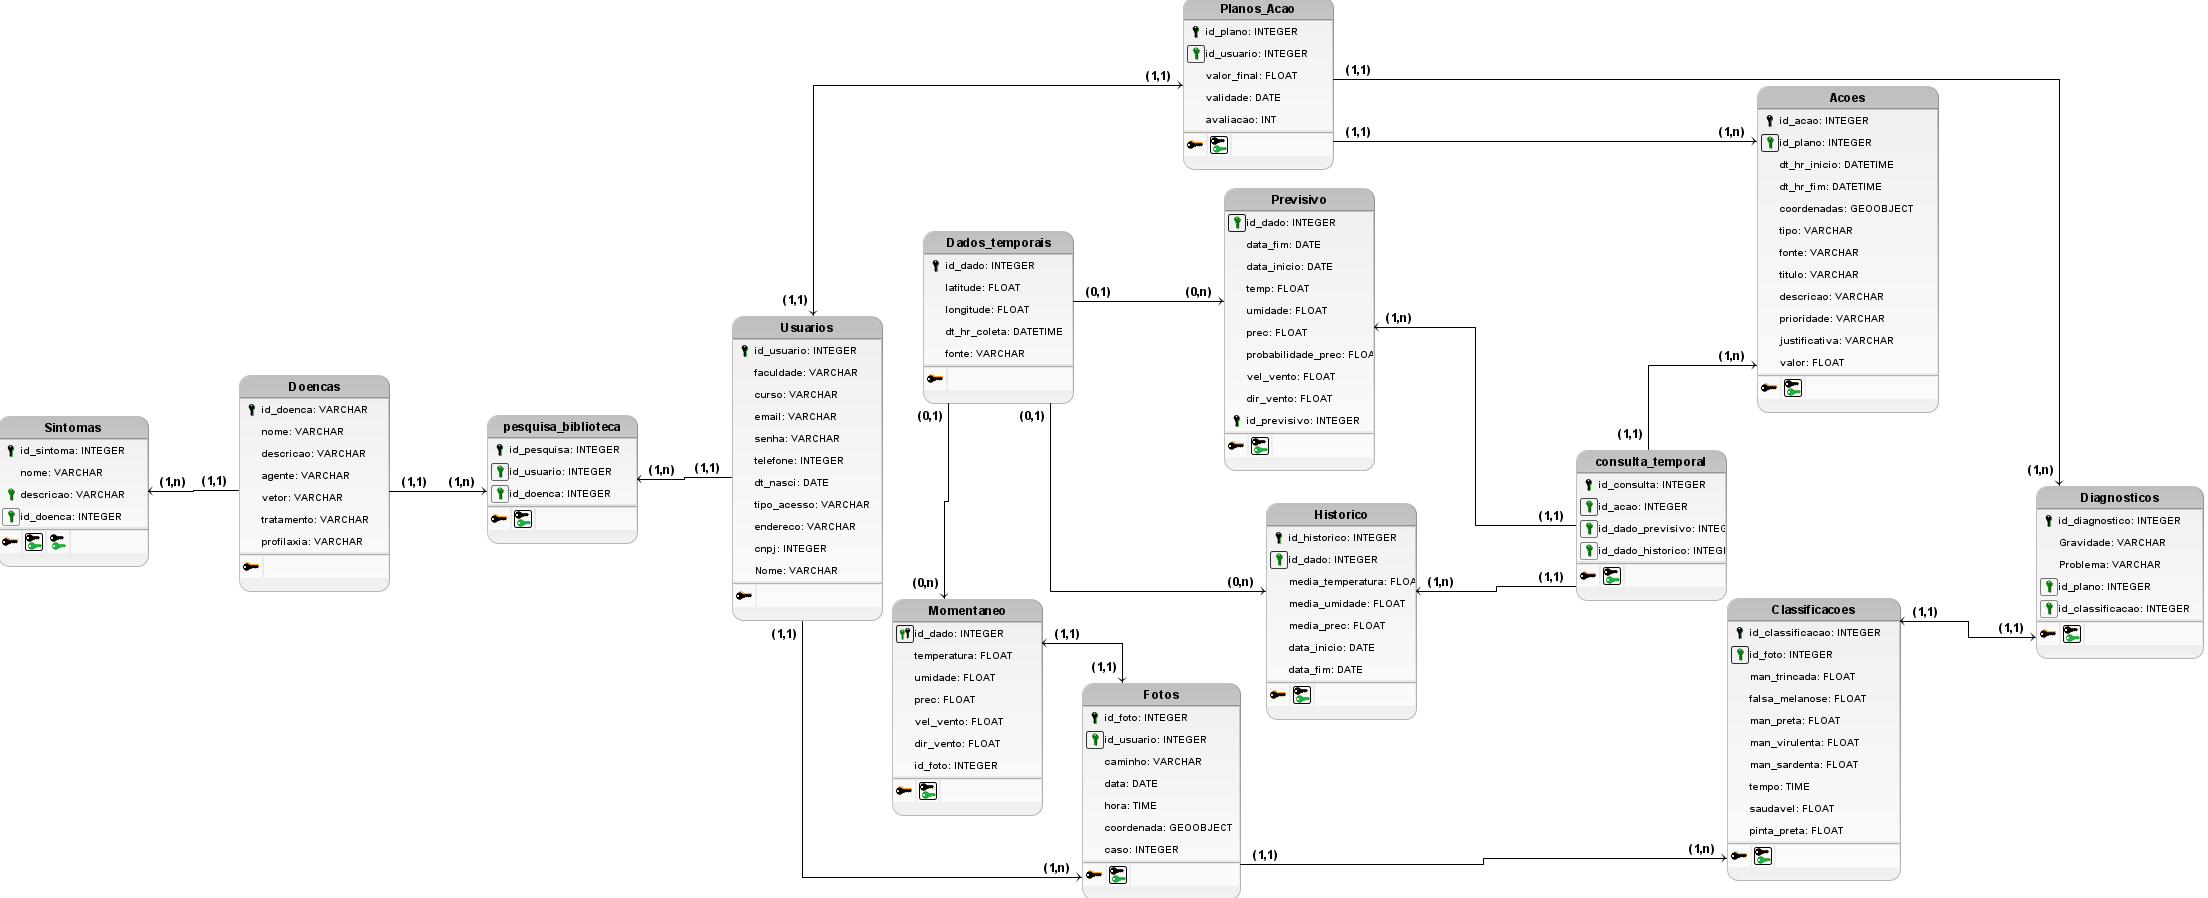
\includegraphics[width=1.0\textwidth]{Logos/logico.png}
\SourceOrNote{Do próprio autor (2025)}
\end{figure}

    Note que as entidades associativas servem apenas para armazenar as chaves das entidades que estão se relacionando, uma vez que os atributos importantes já estão presentes nessas entidades.

\end{document}